\documentclass{article}
\usepackage[pdftex]{graphicx}
\usepackage{amsmath}
\usepackage{verbatim}
\author{Michael Anderson}
\title{Homework Set 5}
\begin{document}
\maketitle
\center{CS533}
\center{Prof. Fern}\\
\flushleft
\newpage

\begin{enumerate}
\item[\textbf{1.}]
Consider the following MDP:

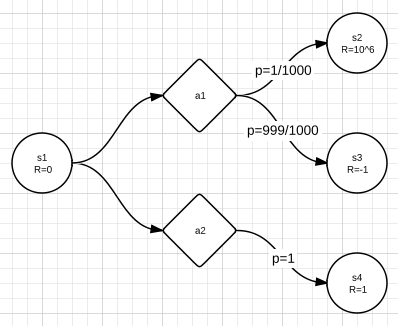
\includegraphics{mdp.png}

Suppose that the given algorithm initially chooses to take action $a_1$ from
state $s_1$. Chances are that it will end up in $s_3$, and receive a negative
reward. Since $s_4$ and the action $a_2$ have a zero reward, and then a 
positive reward once explored, the algorithm
will choose $a_2$ from state $s_1$ from then out. This is because the algorithm
offers no means for exploration. This is a sub-optimal policy, however, because over an
arbitrarily large number of trials $\pi(s_1) \rightarrow (a_1)$ is superior
due to the large reward at the improbable state $s_2$.

\item[\textbf{2.}]
The given $\hat{U}(x,y)$ is linear in all of $(\theta_0,\theta_1,\theta_2,\theta_3)$, so:

\[
\theta_i \leftarrow \theta_i + \alpha(u(s)-\hat{U}(s))
 \frac{\partial \hat{U}(s)}{\partial \theta_i}
\]

And now:

\[
\theta_0 \leftarrow \theta_0 + \alpha(u(s)-\hat{U}(s))
\]

\[
\theta_1 \leftarrow \theta_1 + \alpha(u(s)-\hat{U}(s))(x)
\]

\[
\theta_2 \leftarrow \theta_2 + \alpha(u(s)-\hat{U}(s))(y)
\]

\[
\theta_3 \leftarrow \theta_3 + \alpha(u(s)-\hat{U}(s))\sqrt{(x-x_g)^2 + (y-y_g)^2}
\]

\end{enumerate}
\end{document}
